
\documentclass{article}

\usepackage[pdfborder={0 0 0}]{hyperref}
\usepackage{tikz}

\begin{document}

\title{Unified Memory Heterogenous Computing Showcase}

\maketitle

\section{Frame Execution Overview}

{
	\scriptsize
	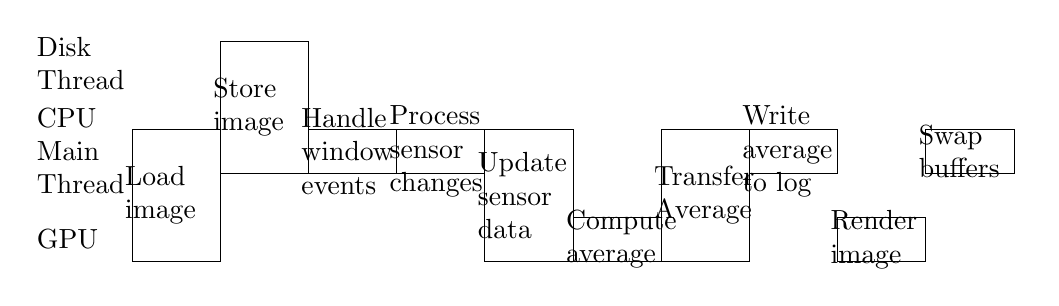
\begin{tikzpicture}[scale=1.12]
		\node[text width=1.3cm] at (-0.5, 1.25) {GPU};
		\node[text width=1.3cm] at (-0.5, 2.25) {CPU Main Thread};
		\node[text width=1.3cm] at (-0.5, 3.25) {Disk Thread};
		\draw[black] (0, 1) rectangle node[text width=1.3cm] {Load image} (1, 2.5);
		\draw[black] (1, 2) rectangle node[text width=1.3cm] {Store image} (2, 3.5);
		\draw[black] (2, 2) rectangle node[text width=1.3cm] {Handle window events} (3, 2.5);
		\draw[black] (3, 2) rectangle node[text width=1.3cm] {Process sensor changes} (4, 2.5);
		\draw[black] (4, 1) rectangle node[text width=1.3cm] {Update sensor data} (5, 2.5);
		\draw[black] (5, 1) rectangle node[text width=1.3cm] {Compute average} (6, 1.5);
		\draw[black] (6, 1) rectangle node[text width=1.3cm] {Transfer Average} (7, 2.5);
		\draw[black] (7, 2) rectangle node[text width=1.3cm] {Write average to log} (8, 2.5);
		\draw[black] (8, 1) rectangle node[text width=1.3cm] {Render image} (9, 1.5);
		\draw[black] (9, 2) rectangle node[text width=1.3cm] {Swap buffers} (10, 2.5);
	\end{tikzpicture}
}

\end{document}
